\chapter {Management API}

Basebox is a SDN controller used in data centers, which are a mission critical component for network operators. As such, management capabilities so that managing
and operating infrastructure must be a central component of this system. There are several steps necessary to understand the problem and be able to choose the most
appropriate design. In this chapter we present the information required to build this system:

\begin{itemize}
    \item Understanding and organizing the information available on the network controllers according to a set of data models;
    \item Analyse the available protocols for handling the transport between the network controllers and the Graphical User Interface;
    \item Decide on the GUI server back-end, and how the visual interface should look like.
\end{itemize}

\section {Data models}

Data models are abstract concepts that map the properties of entities and organizes their attributes, and how they relate to each other. To create a switch 
management interface, the entities we want to model are the switches themselves, with attributes like the switch name, port counters, and the relationships of the 
data will allow us to display the links and topology of the network. One of the considerations that were taken into account when choosing the data models was the
compatibility with standardized data models by the organizational entities like the IETF \footnote{https://www.ietf.org/} and OpenConfig 
\footnote{http://openconfig.net/}.

\par The \textit{NETCONF} \cite{enns_network_2011} network configuration model, which we explore further in \ref{sec:netconf} also defines a data modelling language 
known as \textit{YANG}, which is used in this protocol to model its configuration and data, and the remote procedure calls \cite{bjorklund_yang_2010}. 
YANG data model defines the hierarchy of data between a NETCONF client and server with the objective of smooth integration with the existing system's infrastructure. 

\par The systems we aim to model are two: the topology between the servers and switches, and the port statistics for each port one the switch. Since there is no 
data model that would accurately describe both of them correctly, for the topology we chose the IETF network data model  \cite{clemm_data_2017}, and for the port
counters the OpenConfig interfaces data model \footnote {http://ops.openconfig.net/branches/master/docs/openconfig-interfaces.html}.

\subsection {Topology}

The topology data model maps a collection of nodes, and the relationships between each node, called a link. This also allows for describing the network in a vertical
hierarchy, by displaying relationships between several layers, which can then be used to display the entire networking stack, for example displaying the physical
links between nodes, their connections at layer 2 and layer 3 of the OSI model, and the virtualised relationships that the elements could have in a cloud deployment.
As the development of the product continues, and more features are added, for example, layer 3 routing, then we require a flexible data model that can be extended to
support the new capabilities.

\begin{figure} [!htbp]
    \centering
    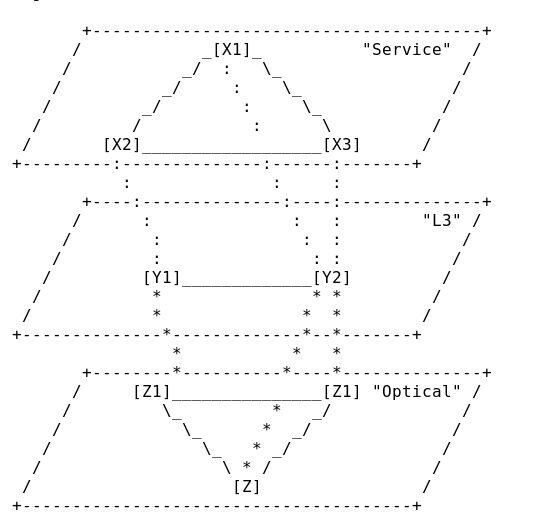
\includegraphics[width=.5\textwidth]{bisdn/network_stack_topologies}
    \caption{Example topology hierarchy achievable with this data model \cite{clemm_data_2017}}
    \label{fig:netconf_stack}
\end{figure}

\par Mapping the data model to the real world data is then adding the two types of information the data model expects: the first one composed of adding the different
networks that composed the entire topology, including their nodes and network types; and then using the previous information to build the links between each of the
nodes, using the termination points the model exposes. As seen in \ref{fig:netconf_stack}, this data model can be extended by adding underlying networks, 
representing the several layers in the networking stack.

\par Displaying the topology proved useful for CAWR since this controller is directly connected to the underlying switches and can see the links among these
networking devices. The connection to the servers can also be monitored, by configuring LACP on the servers interface to report their status. Figure 
\ref{fig:ietf_topology} presents this entire data model, as defined by the IETF.

\begin{figure} [h]
    \centering
    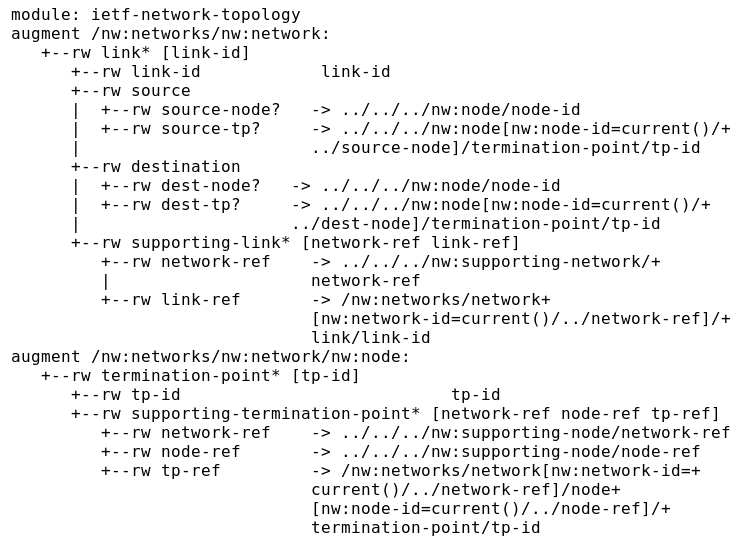
\includegraphics[width=0.7\textwidth]{bisdn/ietf_node}
    \caption{The IETF description for the nodes and links in the proposal for network topologies \cite{clemm_data_2017}}
    \label{fig:ietf_topology}
\end{figure}

\subsection {Port statistics}

\par Modelling the port statistics to build a management interface requires first understanding of the OpenFlow statistics. As mentioned in section \ref{sec:of}, OF
switches maintain a set of counters, similar to SNMP, that provide information about the state of the ports, group, flow and table stats. The statistics that are
exposed from OF are shown in table \ref{tab:of_port_stats}.

\begin{table}[H]
    \centering
    \caption{OpenFlow port statistics}
    \begin{tabular}{c | c || c | c}
       uint64\_t & rx\_packets     & uint64\_t & tx\_packets;     \\ \hline
       uint64\_t & rx\_bytes;      & uint64\_t & tx\_bytes;       \\ \hline
       uint64\_t & rx\_bytes;      & uint64\_t & tx\_dropped;     \\ \hline
       uint64\_t & rx\_errors;     & uint64\_t & tx\_errors;      \\ \hline
       uint64\_t & rx\_frame\_err; & uint64\_t & tx\_over\_err;   \\ \hline
       uint64\_t & rx\_crc\_err;   &                              \\ \hline
       uint64\_t & collisions;     &                              \\ \hline
       uint32\_t & duration\_sec;  &                              \\ \hline
       uint32\_t & duration\_nsec; &                 
    \label{tab:of_port_stats}
    \end{tabular}
\end{table}

\par The chosen data model should then accurately model the fields that we need to expose, and the data type of counters we wish to measure. In this case,
the prevalence of other controllers allows to use the same data models present in their implementations. OpenConfig maintains a set of vendor neutral data models,
written in YANG, allowing network operators to use standardized models for their networking infrastructure. The entire set of published models can be accessed in
their github page \footnote {https://github.com/openconfig/public}.

\section{Protocols}

None of the controllers had a clear way of obtaining the statistics apart from manually looking in the terminal and following the logs exposed and waiting for the
appropriate output. In this section we describe the two \textit {Remote Procedure Call (RPC)} systems that were researched, and focus on the advantages which led 
to the final decision of implementing gRPC on Basebox.

\subsection{NETCONF} \label{sec:netconf}

\par IETF developed a protocol that allowed for installation, manipulation and deletion of configuration of networking devices called NETCONF, which
devices use to expose a full API to their systems. This protocol is set in a client/server communications pattern and is based in the four layers, as can be seen in
the image \ref{fig:netconf_proto_layers}. Data models and operations, covered in detail in the previous section, are related to the Content layer on the image.

\begin{figure} [!htbp]
    \centering
    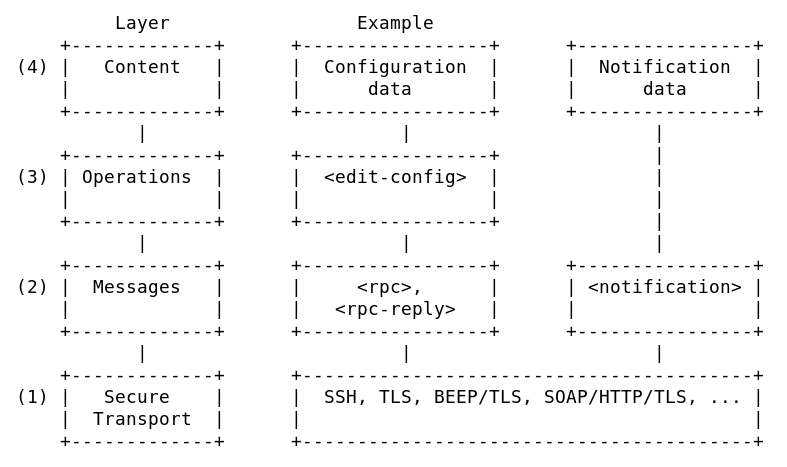
\includegraphics[width=.6\textwidth]{bisdn/netconf}
    \caption{NETCONF protocol layers \cite{enns_network_2011}}
    \label{fig:netconf_proto_layers}
\end{figure}

\par Configuration of a network device can be complex, and managing separate configurations between device startup and normal operation is a difficult task, but
there is occasional need for this capability. NETCONF defines the existence of different \textit{datastores} to enable this feature, allowing the network operator to
set an initial configuration, used when the device is initialized, and switching to the running datastore when the device is ready to maintain normal operation. This
concept of datastores also enables the creation of a candidate datastores, providing the capability of testing configurations on the network device, checking for any
possible errors, while making sure that there is no impact on the current configuration of the device. After the changes have been tested and validated, a <commit>
operation can be used to deploy the new configuration to the running datastore.

\par Another useful feature of the NETCONF protocol, is the possibility of using the rollback-on-error capability. When rolling a new change,
and if the system is enabled to support this feature, NETCONF can detect errors in the changes done to the configurations, and return the system to the previous
state that is error free. 

\par The NETCONF API provides several operations to interact with the managed devices to get system information and push new configurations. The set of supported 
operations in the base NETCONF protocol are \cite{enns_network_2011}:

\begin{table}[H]
    \centering
    \caption{NETCONF Operations}
    \begin{tabular}{c}
       get  \\ \hline
       get-config  \\ \hline
       edit-config  \\ \hline
       copy-config  \\ \hline
       delete-config  \\ \hline
       lock  \\ \hline
       unlock  \\ \hline
       close-session  \\ \hline
       kill-session  
    \end{tabular}
\end{table}

\par NETCONF is able to run on top of several transport protocols. However, NETCONF requires that a persistent connection is maintained  between devices,
and this connection should be reliable, and support transmission failure. In addition, the security should be handled by the transport layer 
\cite{jurgen_schonwalder_network_2012}, providing the guarantee that transactions are done in a cryptographically secure channel, between two authenticated hosts. 
As a result, typical NETCONF implementations are based on SSH or TLS protocols.

\subsection{gRPC} \label{sec:grpc}

The basic idea behind RPC systems is defining an interaction between remote environments where subroutines are executed as if they were executed as a local
procedure call. These subroutines are defined by specifying the methods that can be called, with their parameters and return values.

\par gRPC defines a data serialization format known as protocol buffers, or \textit {protobuf}, which is used for defining the service interface and the
structure of the messages. This system is based in HTTP/2, due to the optimizations present in this protocol, like

\begin{itemize}
    \item header compression, which reduces overhead in transmission;
    \item multiplexing of multiple requests over single connections;
    \item and stream prioritization, which allows the creation of streaming RPCs, where a bi-directional sequence of messages can be exchanged.
\end{itemize}

\par There are some projects \footnote {https://github.com/openconfig/goyang} that enable the translation between YANG to protobuf, which allows us to use the data
models previously chosen, only adding the extra step to convert the files.

\par Data serialization is a common task for communication between services, and optimization of this task, specifically regarding the speed, allows for reducing
overheads in the transmission of the data. A comparative study regarding several serialization formats reports \cite{maxim_novak_serialization_2014}, without any
optimizations, protobuf improves performance on serializing and de-serializing messages compared to XML or JSON.

\subsection{Comparison}

\par Despite of both protocols capability of meeting the requirements that were presented to us, the gRPC framework was chosen due to several reasons:

\begin {itemize}
    \item Both frameworks allow us to use the standardized data models currently proposed by the IETF and OpenConfig;
    \item NETCONF trades information as XML encoded information; while gRPC allows to handle information in a way that’s native to the language implementation 
        of the client/server;
    \item The integration with the existing system was easier: since gRPC has implementations for the languages that the controllers are developed on
        (i.e. C++), this framework was easier to implement than NETCONF, which would have required integration with third party tools.
\end {itemize}

\section {Implementation}

\begin{figure}
    \centering
    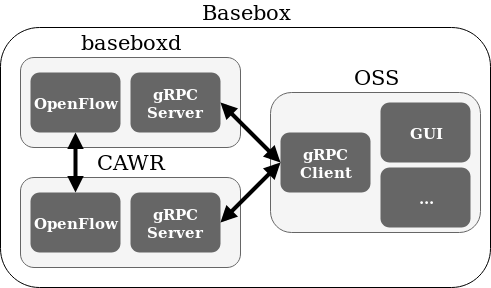
\includegraphics[width=.6\textwidth]{bisdn/prp_system_low_level}
    \caption{Operations Support System architecture}
    \label{fig:oss}
\end{figure}

By combination of the technologies presented in this chapter, we have developed an Operations Support System (OSS), visible in figure \ref{fig:oss}. 

\subsection{Proof-of-concept}

Able to connect to baseboxd and CAWR

draw the physical node topology, and display the port statistics. This GUI can be accessed via a web page, since this provides an ease of access to the system. 
The web page was developed on top of the Django Framework \footnote{\url{https://www.djangoproject.com/}}, due to the Python implementation, support for official
gRPC integration and ease of implementation. For drawing the topology we used the JavaScript library D3.js \footnote{\url{https://d3js.org/}}.

\begin{figure} [H]
        \centering
        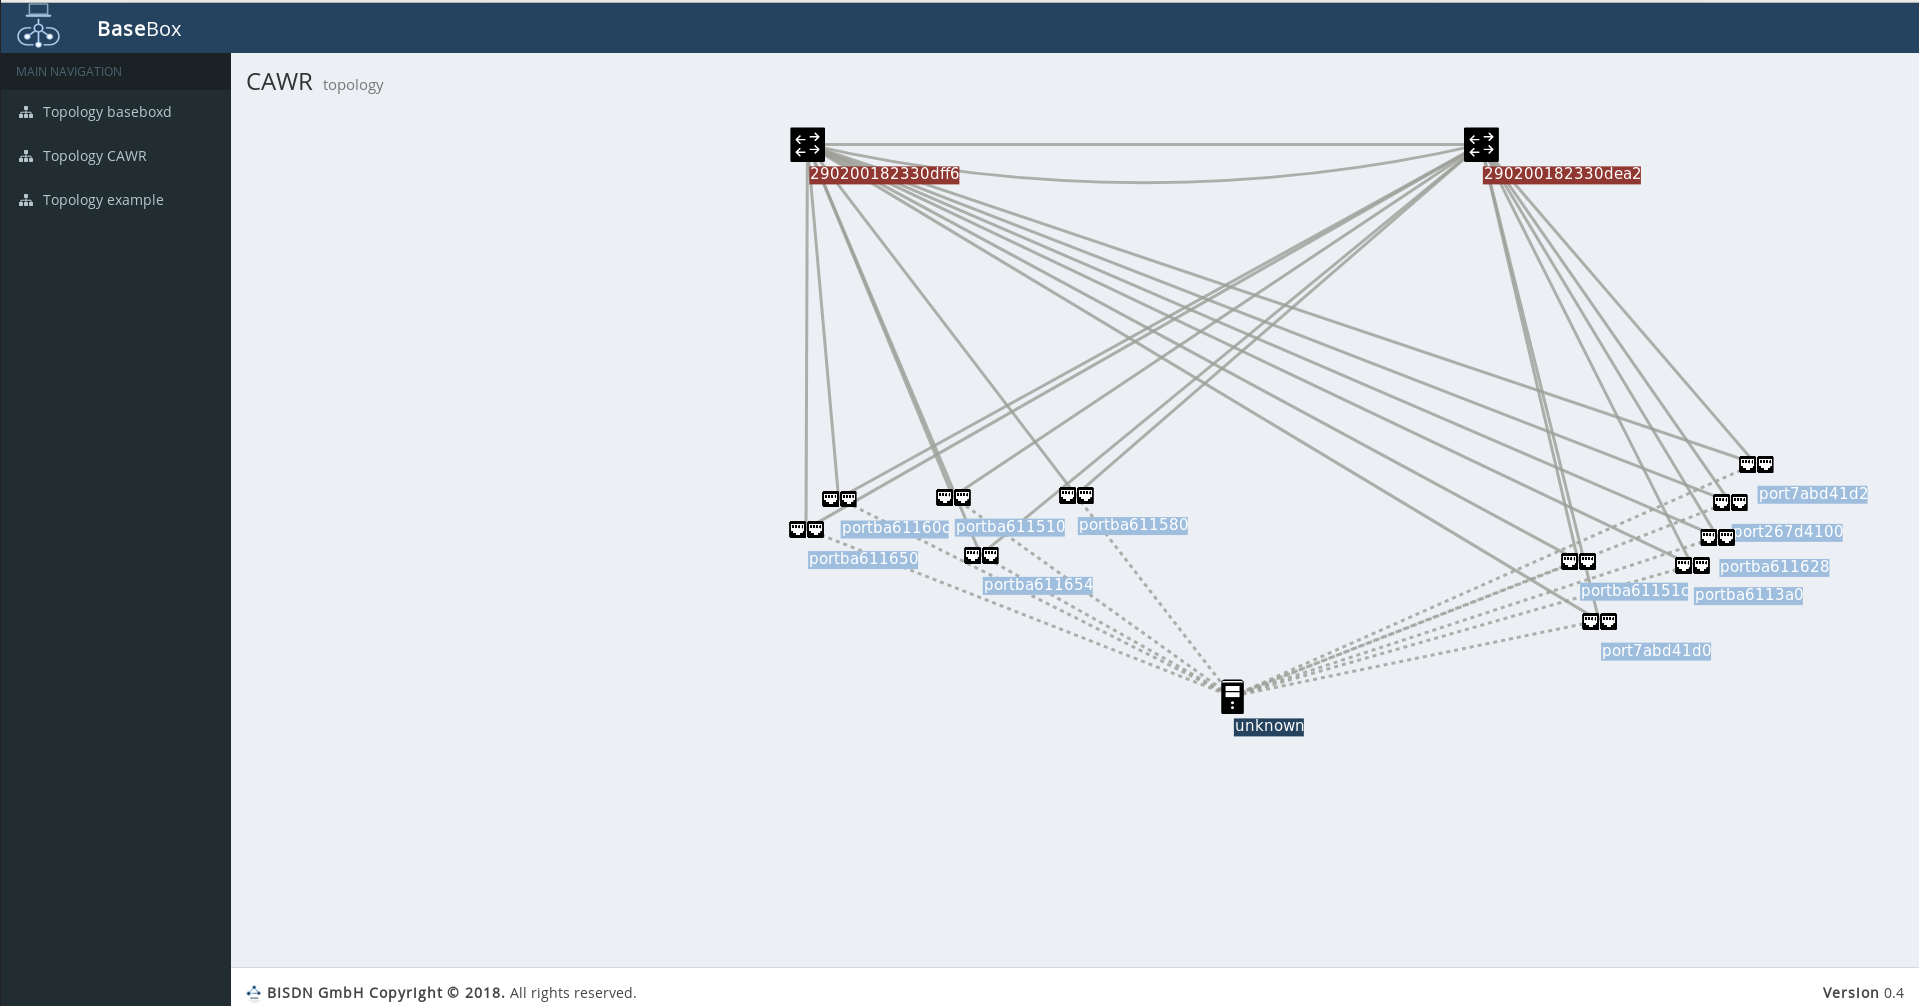
\includegraphics[width=.7\textwidth]{bisdn/cawr_gui}
        \caption{Topology obtained from CAWR}
        \label{fig:cawr_gui}
\end{figure}

\begin{figure}
    \centering
    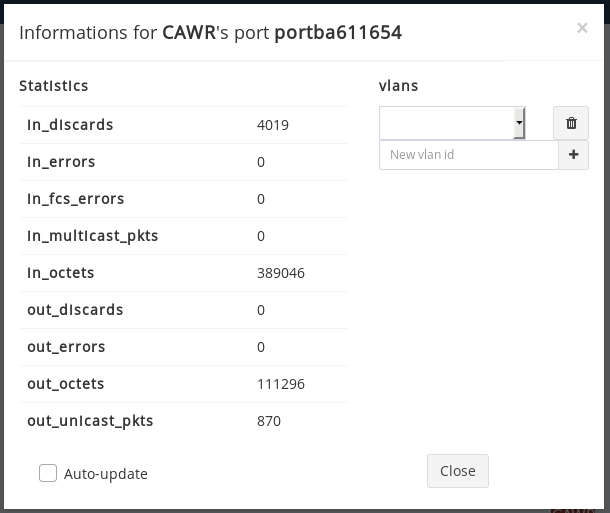
\includegraphics[width=.5\textwidth]{bisdn/basebox_gui}
    \caption{Single Port statistics from Baseboxd}
\end{figure}

\par Figure \ref{fig:cawr_gui} displays the topology that CAWR reports, and table \ref{tab:gui-mapping} displays the meaning of the icons present in the GUI. Since 
this system is to be used in a real time deployment, there is no interest in storing the state of the network, which means that the topology must be drawn with 
every request to the server. Currently the topology is updated every two seconds, providing a balance between real time updates and the interval for requests to the
controllers.

\par The connection between both controllers to the GUI provides the view for both controllers, which means that CAWR will present the view for the physical
switches, bonded ports and hosts, while the baseboxd only shows the giant switch created by CAWR. An advantage of this is the analysis of the global view of the
state of the network, and further possibilities include the addition of displaying configured VLANs in each port, and even provide a way to configure them via a GUI.
Interaction with the nodes is possible, and clicking on each provides an insight to the statistics related to that port.  
